\chapter{Resultados y validación}
\label{cap:capitulo5}

\vspace{1cm}

Una vez finalizado el desarrollo del proyecto, se evalúa la usabilidad de la plataforma mediante una encuesta de satisfacción a los usuarios, quienes valoraron su funcionamiento.\\

Se ha realizado una encuesta con 9 preguntas sobre la experiencia del juego a personas sanas.
Los resultados obtenidos han sido los siguientes (n=9):
\begin{figure}[ht!]
	\centering
	\begin{minipage}{0.75\linewidth}
		\centering
		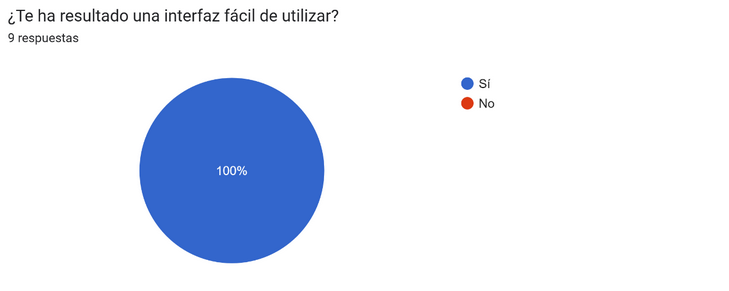
\includegraphics[width=\linewidth]{figs/pregunta1.png}
	\end{minipage}
	\caption[Encuesta de satisfacción. Pregunta 1]{El $100\%$ de los participantes considera que la interfaz es sencilla}
	\label{fig:level1}
\end{figure}

\begin{figure}[ht!]
	\centering
	\begin{minipage}{0.75\linewidth}
		\centering
		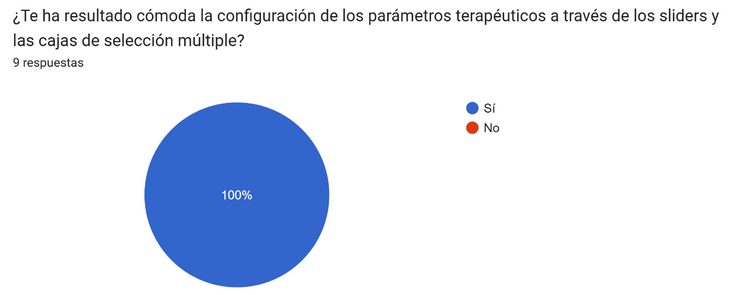
\includegraphics[width=\linewidth]{figs/pregunta2.png}
	\end{minipage}
	\caption[Encuesta de satisfacción. Pregunta 2]{El $100\%$ de los participantes está de acuerdo con que el diseño de la interfaz de control es cómoda de utilizar}
	\label{fig:level2}
\end{figure}

\begin{figure}[ht!]
	\centering
	\begin{minipage}{0.75\linewidth}
		\centering
		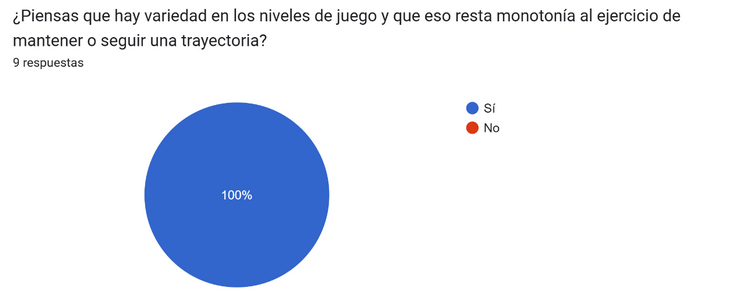
\includegraphics[width=\linewidth]{figs/pregunta3.png}
	\end{minipage}
	\caption[Encuesta de satisfacción. Pregunta 3]{El $100\%$ de los participantes ha votado que hay variedad en los niveles de juego}
	\label{fig:level3}
\end{figure}

\begin{figure}[ht!]
	\centering
	\begin{minipage}{0.71\linewidth}
		\centering
		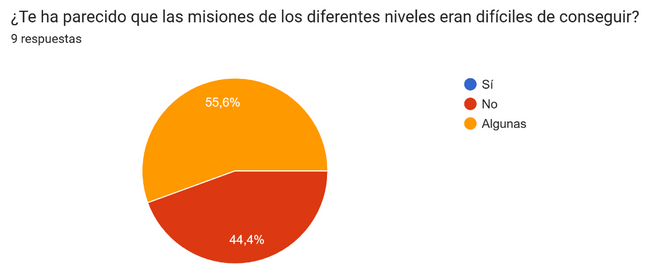
\includegraphics[width=\linewidth]{figs/pregunta4.png}
	\end{minipage}
	\caption[Encuesta de satisfacción. Pregunta 4]{El $55,6\%$ de los participantes piensa que algunas misiones del juego son difíciles de superar y el $44,4\%$ no cree que sean complejas}
	\label{fig:level1}
\end{figure}

\begin{figure}[ht!]
	\centering
	\begin{minipage}{0.85\linewidth}
		\centering
		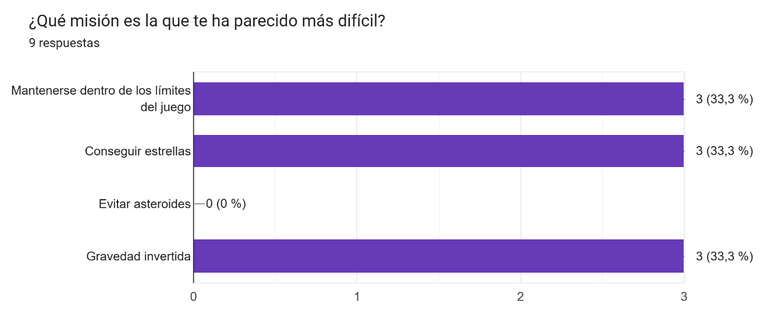
\includegraphics[width=\linewidth]{figs/pregunta5.png}
	\end{minipage}
	\caption[Encuesta de satisfacción. Pregunta 5]{Las misiones más difíciles según los usuarios son: mantenerse dentro de los límites del juego, conseguir estrellas y gravedad invertida}
	\label{fig:level2}
\end{figure}

\begin{figure}[ht!]
	\centering
	\begin{minipage}{0.85\linewidth}
		\centering
		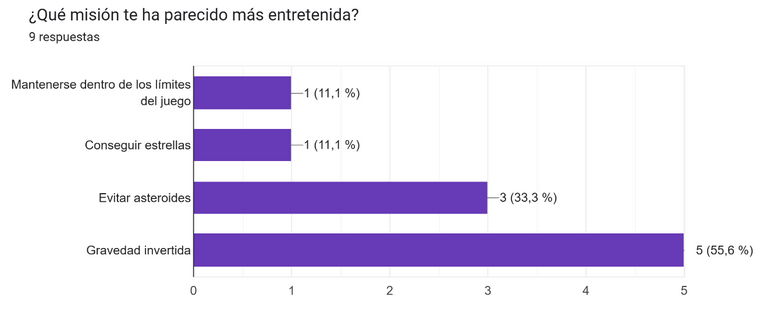
\includegraphics[width=\linewidth]{figs/pregunta6.png}
	\end{minipage}
	\caption[Encuesta de satisfacción. Pregunta 6]{El $55,6\%$ de los participantes ha votado que la misión más entretenida es la de gravedad invertida}
	\label{fig:level3}
\end{figure}

\begin{figure}[ht!]
	\centering
	\begin{minipage}{0.75\linewidth}
		\centering
		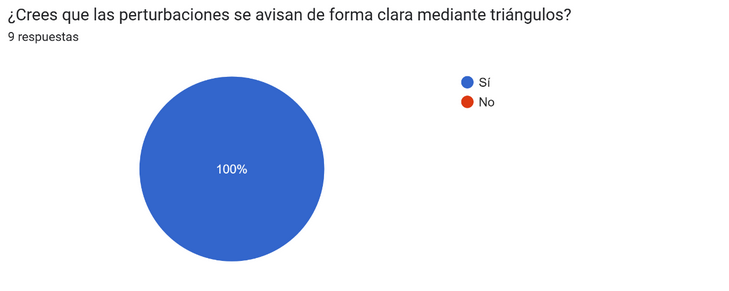
\includegraphics[width=\linewidth]{figs/pregunta7.png}
	\end{minipage}
	\caption[Encuesta de satisfacción. Pregunta 7]{El $100\%$ de los participantes piensa que las perturbaciones están bien señalizadas en el juego}
	\label{fig:level1}
\end{figure}

\begin{figure}[ht!]
	\centering
	\begin{minipage}{0.75\linewidth}
		\centering
		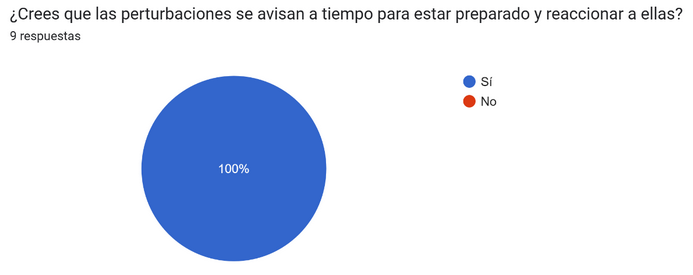
\includegraphics[width=\linewidth]{figs/pregunta8.png}
	\end{minipage}
	\caption[Encuesta de satisfacción. Pregunta 8]{El $100\%$ de los participantes considera que las perturbaciones aparecen con anterioridad antes de que sean notables}
	\label{fig:level2}
\end{figure}

\begin{figure}[ht!]
	\centering
	\begin{minipage}{0.85\linewidth}
		\centering
		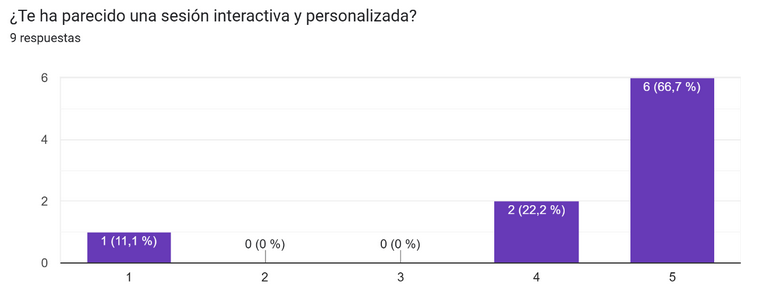
\includegraphics[width=\linewidth]{figs/pregunta9.png}
	\end{minipage}
	\caption[Encuesta de satisfacción. Pregunta 9]{El $66,7\%$ de los participantes ha votado que la sesión terapéutica es interactiva y personalizada}
	\label{fig:level3}
\end{figure}

Como conclusión se refleja que la interfaz del juego es sencilla (el $100\%$ de los participantes así lo consideran), que unas misiones son más entretenidas y difíciles que otras y que las sesiones son interactivas y personalizadas (el $66,7\%$ de los participantes en la encuesta han contestado la mayor puntuación).

Está pendiente realizar la encuesta con pacientes post-ictus.
